\section{Non-linear Systems of ODEs}

Since many differential equations cannot be solved conveniently by analytical methods, it is important to consider what qualitative information can be obtained about their solutions without actually solving the equations. Studying the qualitative theory tells us the general behaviour of the ODE for all possible trajectories. There are two aspects to this theory:
\begin{itemize}
	\item Looking at the ODE locally near $\xta$,
	\item Global aspect across $\R^n$.
\end{itemize}

We will now focus on $\vbx = (x, y) \in \R^2$ where 
\begin{equation}\label{eq:linearsystem2}
	\begin{cases}
		x' = F(x,y) \\
		y' = G(x,y)
	\end{cases}
\end{equation}
Since $F$ and $G$ can be arbitrary, the problem is generally non-linear.

The terminology used here might be useful in the content that follows: the $(x,y)$ plane is a \vb{phase plane}, where vector fields are plotted and a representative set of trajectories is referred to as a \vb{phase portrait}.

\begin{definition}
	A point $\vbx_0 = (x_0, y_0)$ is a \textbf{critical point} if $F(x_0, y_0) = G(x_0, y_0) = 0$.
\end{definition}

\begin{theorem}[Rectification theorem]
	Consider $\xta = (x_{\ast}, y_{\ast})$ such that $(F(\xta), G(\xta)) \neq (0,0)$. Then, in a neighbourhood of $\xta$, there is a smooth change of variables $(x,y) \mapsto (\Tilde{x}, \Tilde{y})$ that transforms the ODE into 
	\[
	\begin{cases}
		\Tilde{x}' = 1 \\
		\Tilde{y}' = 0
	\end{cases}
	\]
\end{theorem}

If $(F(\xta), G(\xta)) = (0,0)$, then $\xta$ is a \vb{critical point}, also known as an equilibrium point or a fixed point. If $\vbx(0) = \xta$, then $\xt = \xta$ for all $t$, since both $x'$ and $y'$ are zero so $x$ and $y$ will not change over time when we start at a critical point.

\subsection{Linear Approximation near a Critical Point}\label{sec:linearapproxcp}

Let $\xta = (x_{\ast},y_{\ast})$ be a critical point. Then $F(\xta) = G(\xta) = 0$. We have the following system of equations:
\[
\begin{cases}
	x(t) = x_{\ast} + u(t) \\
	y(t) = y_{\ast} + v(t)
\end{cases}
\]
where $u(t), v(t)$ are perturbations of $x$ and $y$ respectively.

The system in \Cref{eq:linearsystem2} is locally in the neighbourhood of $\xta$ whenever the functions $F$ and $G$ have continuous partial derivatives up to order two. To show this, we use Taylor expansions about the point $\xta$ to write $F(x, y)$ and $G(x, y)$ in the form:
\[ 
u' = F(x_{\ast} + u, y_{\ast} + v) = F(\xta) + \p_x F(\xta)u + \p_y F(\xta)v + \eta_1 \xt \]
\[
v' = G(x_{\ast} + u, y_{\ast} + v) = G(\xta) + \p_x G(\xta)u + \p_y G(\xta)v + \eta_2 \xt
\]

We can now notice that
\[
\frac{\eta_i}{\Vert \vbx - \xta \Vert} \rightarrow 0 \text{ as } \vbx \rightarrow \xta,
\]
and since $F(\xta) = G(\xta)=0$, we now have a linear system of ODEs of the form
\begin{equation}\label{3.2}
	\mat{u'\\v'} = \mat{\p_x F(\xta) & \p_y F(\xta) \\ \p_x G(\xta) & \p_y G(\xta)} \mat{u\\v},
\end{equation}
where $J = \mat{\p_x F(\xta) & \p_y F(\xta) \\ \p_x G(\xta) & \p_y G(\xta)}$ is called the \vb{Jacobian matrix}.

Since the Jacobian is calculated at the Critical point $\xta$, it is a constant matrix that gives a linear system that can be solved using methods from \Cref{sec:firstorder}.

\begin{eg}[Damped Pendulum]\label{eg:dampedpendulum} Consider the equations:
	\begin{align*}
		x' &= y = F(\xta)\\
		y' &= -\omega^2 \sin{x} - \gamma y = G(\xta)
	\end{align*}
	(For the physicists out there, $\omega = \sqrt{\frac{g}{L}}$, where $g$ is the gravitational constant, $L$ is the length of the pendulum, and $\gamma$ is the friction coefficient)
	
	We find the critical points ($x'=y'=0$) to be:
	\[
	y=0 
	\]
	\[
	-\omega^2 \sin{x} - \gamma y = 0 \implies -\omega^2 \sin{x} = 0 \implies\sin{x} = 0 \implies x = n\pi
	\]
	where $n \in \Z$. We find the Jacobian to be given by:
	\[
	J(x,y) = \mat{
		\p_x F(\xta) & \p_y F(\xta) \\ \p_x G(\xta) & \p_y G(\xta)} = \mat{ 0 & 1 \\ 
		-\omega^2 \cos{x} & -\gamma}
	\]
	At the critical points, 
	\[
	J(n\pi,0) = \mat{ 0 & 1 \\ -\omega^2(-1)^n & -\gamma}
	\]
	which depends on the value of $n$ as $\cos{x} = -1$ for odd $n$ and $\cos{x} = 1$ for even $n$. The system is now given by 
	\[
	\mat{u'\\v'} = \mat{0 & 1 \\ -\omega^2(-1)^n & -\gamma} \mat{u\\v}
	\]
	which can be solved using \Cref{sec:firstorder} (left as an exercise for the reader).
	
	A vector field generated in Python in the style of \Cref{fig:geomsys} is shown in \Cref{fig:pendulumpython}.
\end{eg}

\begin{figure}[H]
	\centering
	\includegraphics[width=0.7\textwidth]{vectorFieldPendulum.pdf}
	\caption{Direction field and selected solution trajectories for the damped pendulum.}
	\label{fig:pendulumpython}
\end{figure}

\subsection{Classification of Critical points}

We now consider 2-dimensional systems of the form: 
\[
\begin{cases}
	x' = F(x,y) \\
	y' = G(x,y) 
\end{cases}
\]

For the critical point $\xta = (x_{\ast}, y_{\ast})$, let $x(t) = x_{\ast} + u(t)$ and $y(t) = y_{\ast} + v(t)$. As seen above, we have a linearised system for $\mat{u'\\v'}$ as given in \Cref{3.2}. So upon solving, $\mat{u'\\v'}$ we have solutions of the form: 
\begin{equation}\label{3.5}
	\mat{u(t)\\v(t)} = 
	c_1 e^{r_1t} \xib_1 + c_2 e^{r_2t} \xib_2
\end{equation}
where $r_1, r_2$ are the eigenvalues of the Jacobian matrix $J(x,y)$ and $\xib_1, \xib_2$ are the associated eigenvectors.

Using these eigenvalues, we can predict the behaviour of the ODEs near critical points (see \Cref{table:stability} for a summary).
\begin{itemize}
	\item Case 1: Real Unequal Eigenvalues:
	\begin{enumerate}[label=(\roman*)]
		\item $r_1 < r_2 < 0$: \\
		Consider the solution $\xt = c_1 e^{r_1t} \xib_1 + c_2 e^{r_2t} \xib_2 = e^{r_2t} (c_1 e^{(r_1-r_2)t} \xib_1 + c_2 \xib_2)$. \\
		We now observe how $x$ changes as $t \to \pm \infty$: \\
		\underline{As $t \to \infty$}: if $c_2 \neq 0$, then the term $c_1 e^{(r_1-r_2)t} \xib_1$ is of negligible magnitude compared to $c_2 \xib_2$ for sufficiently large $t$, so $\xt \to 0$ along $\xib_2$.
		If $c_2 = 0$ (i.e. the solution starts on the line $\xib_1$) then $\xt \to 0$ along $\xib_1$. \\
		\underline{As $t \to -\infty$}: if $c_1 \neq 0$, then the dominant term is $c_1 e^{r_1t} \xib_1$ and $\xt \to \infty$ along $\xib_1$. 
		If $c_1 = 0$, then $|\xt| \to \infty$ along $\xib_2$. \\
		The critical point in this case is a \vb{nodal sink} (see \Cref{fig:trajectory1}).
		
		\item $r_1 > r_2 > 0$: \\
		Consider the solution $\xt = c_1 e^{r_1t} \xib_1 + c_2 e^{r_2t} \xib_2$. \\
		We now observe how $x$ changes as $t \to \pm \infty$: \\
		\underline{As $t \to \infty$}: if $c_1 \neq 0$, then $|\xt| \to \infty$ along $\xib_1$ as the $c_1 e^{r_1t} \xib_1$ term dominates.
		If $c_1 = 0$, then $|\xt| \to \infty$ along $\xib_2$. \\
		\underline{As $t \to -\infty$}: if $c_2 \neq 0$, then $\xt \to 0$ along $\xib_2$ as the $c_2 e^{r_2t} \xib_2$ term dominates.  
		If $c_2 = 0$, then $\xt \to 0$ along $\xib_1$. \\
		The critical point in this case is a \vb{nodal source} (essentially the same as \Cref{fig:trajectory1}, with the arrows all running in the opposite direction).
		
		\item $r_1 > 0 > r_2$: \\
		Consider the solution $\xt = c_1 e^{r_1t} \xib_1 + c_2 e^{r_2t} \xib_2$. \\
		We now observe how $x$ changes as $t \to \pm \infty$: \\
		As $t \to \infty$, the $c_1 e^{r_1t}\xib_1$ term dominates and $|\xt| \to \infty$. As $t \to -\infty$, the $c_2 e^{r_2t}\xib_2$ term dominates and $|\xt| \to \infty$ also. \\
		The exceptions are: \\
		$c_1 = 0$, in which case $x \to0$ as $t \to \infty$ since $r_2$ is negative. \\
		$c_2 = 0$, in which case $x \to0$ as $t \to -\infty$. \\
		The critical point in this case is a \vb{saddle point} (see \Cref{fig:trajectory2}).
	\end{enumerate}
	
	\begin{figure}[H]
		\centering
		\includegraphics[width=0.5\textwidth]{Trajectories/1.pdf}
		\caption{Trajectories in the phase plane when the origin is a node (nodal sink) with $r_1 < r_2 < 0$. The solid black and dashed black curves show the fundamental solutions $\xib^{(1)}e^{r_1t}$ and $\xib^{(2)}e^{r_2t}$, respectively \cite[Figure 9.1.1]{boyce}.}
		\label{fig:trajectory1}
	\end{figure}
	
	\begin{figure}[H]
		\centering
		\includegraphics[width=0.53\textwidth]{Trajectories/2.pdf}
		\caption{Trajectories in the phase plane when the origin is a saddle point with $r_2 < 0 < r_1$. Note that the trajectories along one of the eigenvectors approach zero (this is the eigenvector associated with the negative eigenvalue), while those along the other eigenvector tend to $\infty$. \cite[Figure 9.1.2]{boyce}.}
		\label{fig:trajectory2}
	\end{figure}
	
	\item Case 2: Complex Eigenvalues of the form $r = \lambda \pm i \mu$ ($\mu>0$):
	
	A system with these eigenvalues can be transformed into the system:
	\begin{equation}\label{3.6}
		\xtp = \mat{ \lambda & \mu \\ -\mu & \lambda} \xt
	\end{equation} 
	and the solution to this system is given by:
	\[
		\xt = c_1 e^{\lambda t} \mat{\cos{\mu t} \\ -\sin{\mu t}} + c_2 e^{\lambda t} \mat{\sin{\mu t} \\ \cos{\mu t}} 
	\]
	as seen in \Cref{sec:complexeigs}. We now consider the following two subcases: 
	\begin{enumerate}[label=(\roman*)]
		\item $\lambda \neq 0$: \\ 
		From \Cref{3.6}, we have 
		\begin{align*}
			x' &= \lambda x + \mu y \\
			y' &= -\mu x + \lambda y
		\end{align*}
		Changing to polar coordinates, let $x= r \cos{\theta}, y = r \sin{\theta}$. Differentiating $x,y$ and Substituting the $x,y$ values into the equations above, we get: 
		\begin{equation}\label{eq3.7}
			x' = r'\cos{\theta} - r\theta'\sin{\theta} = \lambda r \cos{\theta} + \mu r\sin{\theta}
		\end{equation}
		\begin{equation}\label{eq3.8}
			y' = r'\sin{\theta} + r\theta'\cos{\theta} = -\mu r \cos{\theta} + \lambda r\sin{\theta}
		\end{equation}
		Multiplying \Cref{eq3.7} by $\cos{\theta}$ and \Cref{eq3.8} by $\sin{\theta}$, and adding the two equations, we get: 
		\[
		r' = \lambda r
		\]
		Multiplying \Cref{eq3.7} by $-\sin{\theta}$ and \Cref{eq3.8} by $\cos{\theta}$, and adding the two equations, we get: 
		\[
		\theta' = -\mu
		\]
		As $t \to \infty$, $r \to 0$ if $\lambda<0$ and $r \to \infty$ if $\lambda>0$. 
		The critical point in this case is a \vb{spiral sink} (\vb{stable focus}) when $\lambda<0$ and \vb{spiral source} (\vb{unstable focus}) when $\lambda>0$ (see \Cref{fig:trajectory5}). 
		% Since $\theta' = -\mu$, if $\mu>0$ then $\theta$ decreases as $t$ evolves and the motion is clockwise; if $\mu<0$ the trajectories are traversed anticlockwise.
		
		\item $\lambda = 0$: \\
		With the equations in subcase (i) holding, we now have that $r'=0 \implies r$ is constant so the trajectories are circles in the transformed coordinates. It can be shown that the trajectories are ellipses in the original coordinates, so the critical point in this case is a \vb{centre}, as in \Cref{fig:trajectory6}.
	\end{enumerate}

	To determine whether motion is clockwise or anticlockwise, we must look to the original linear system,
	\[
		\xtp = \mat{a & b \\ c & d}\xt.
	\]
	If $b-c>0$, the motion is clockwise; if $b-c<0$, the motion is anticlockwise.
	
	\begin{figure}[h!]
		\centering
		\includegraphics[width=0.8\textwidth]{Trajectories/5.pdf}
		\caption{Trajectories in the phase plane for a linear system with eigenvalues $\lambda \pm i\mu$, where the origin is (a) a spiral sink with $\lambda <0$ and (b) a spiral source with $\lambda >0$ \cite[Figure 9.1.5]{boyce}.}
		\label{fig:trajectory5}
	\end{figure}
	
	\begin{figure}[h!]
		\centering
		\includegraphics[width=0.5\textwidth]{Trajectories/6.pdf}
		\caption{Trajectories in the phase plane for a linear system with eigenvalues $\pm i\mu$, where the origin is a centre \cite[Figure 9.1.6(a)]{boyce}.}
		\label{fig:trajectory6}
	\end{figure}
	
	\item Case 3: Real and Equal Eigenvalues $r_1 = r_2 = r < 0$:
	
	For cases with repeated eigenvalues, recall that as seen in \Cref{sec:repeatedeigs}, we can either have 2 or 1 linearly independent eigenvectors associated with $r$ depending on the geometric multiplicities of the eigenvalues. We consider the following two subcases:
	\begin{enumerate}[label=(\roman*)]
		\item Two linearly independent eigenvectors: \\ 
		The solution is given by 
		\[
		\xt = c_1 e^{rt} \xib_1 + c_2 e^{rt} \xib_2
		\]
		The ratio $\frac{x}{y}$ is independent of $t$ but depends on the components of $\xib_1$ and $\xib_2$ and on $c_1, c_2$. Thus every trajectory lies on a straight line through the origin and since $r<0$, the trajectories approach the critical point as $t \to \infty$. The critical point in this case is a \vb{proper node} (\vb{star point}) (see \Cref{fig:trajectory3}).
		
		\item One linearly independent eigenvector: \\
		The solution is given by 
		\[
		\xt = c_1 e^{rt} \xib + c_2 e^{rt} (\xib t + \etab)
		\]
		Since $r<0$, the trajectories approach the critical point. As $t \to \infty$, the trajectory is dominated by $\xib$ (if $c_2 \neq 0$, the $c_2 te^{rt} \xib$ term dominates; if $c_2 = 0$ then $c_1 e^{rt} \xib$ dominates) so approaches the origin tangent to the line through this eigenvector. The critical point in this case is an \vb{improper node}, or \vb{degenerate node} (see \Cref{fig:trajectory4}).
		
		As in the case for complex eigenvalues, if $b-c>0$, the motion is clockwise; if $b-c<0$, the motion is anticlockwise.\footnote{If $b-c=0$, the critical point cannot be a spiral, centre, or improper node.}
	\end{enumerate}
	If instead the eigenvalues are positive, $r_1 = r_2 = r > 0$, the trajectories are similar but the direction of motion is reversed.
\end{itemize}

\begin{figure}[h!]
	\centering
	\includegraphics[width=0.5\textwidth]{Trajectories/3.pdf}
	\caption{Trajectories in the phase plane when the origin is a proper node with $r_1 = r_2 < 0$ \cite[Figure 9.1.3(a)]{boyce}.}
	\label{fig:trajectory3}
\end{figure}

\begin{figure}[h!]
	\centering
	\includegraphics[width=0.8\textwidth]{Trajectories/4.pdf}
	\caption{Trajectories in the phase plane when the origin is (a) an improper node with eigenvalues $r_1 = r_2 < 0$ and one independent eigenvector $\xib$, and (b) the same but with a different generalised eigenvector $\etab$ \cite[Figure 9.1.4]{boyce}.}
	\label{fig:trajectory4}
\end{figure}

\subsection{Stability of Critical Points and Systems}

We know that if $\vbx(0) = \xta$, then $\xt = \xta$ for all $t$. Now we consider what happens to trajectories starting near $\xta$.

\begin{definition}
	A critical point $\xta$ is \vb{stable} if $\forall \varepsilon>0$, $\exists \delta>0$ such that $|\vbx(0) - \xta| < \delta$ implies $|\xt - \xta|<\varepsilon$ for all $t>0$.
\end{definition}

\begin{definition}
	A critical point $\xta$ that is not stable is called unstable.
\end{definition}

\begin{definition}
	A critical point $\xta$ is \vb{asymptotically stable} if it is stable and $\exists \delta_0 >0$ such that $|\vbx(0) - \xta| < \delta_0$ implies $|\xt - \xta|<\varepsilon$ as $t \to \infty$.
\end{definition}

Intuitively, a critical point being stable means that, starting from a point close to the critical point, the trajectory remains close to the point. A CP being asymptotically stable means that, starting close to the CP, the trajectory will tend towards the critical point.

A graphical representation of stability and asymptotic stability is given in \Cref{fig:stability}.

\begin{figure}[!ht]
	\centering
	\includegraphics[width=0.75\textwidth]{stability.pdf}
	\caption{Graphical representation of trajectories that exhibit (a) asymptotic stability and (b) stability \cite[Figure 9.2.1]{boyce}.}
	\label{fig:stability}
\end{figure}

\subsubsection{Stability of Linear Systems}

We already know that for a linear system $\xtp = A\xt$, the solution is given by
\[
\xt = c_1e^{r_1t}\xib_1 + c_2e^{r_2t}\xib_2,
\]
and a critical point is $\xta = (0,0)$.

Stability for a linear system depends on the sign of the eigenvalues:
\begin{itemize}
	\item If $\Re(r_1) \leq 0$ and $\Re(r_2) \leq 0$, this implies that the linear system is stable as trajectories will return to the origin (or, at the very least, the trajectories will not go away from the origin) as $e^{r_1t}$ and $e^{r_2t}$ decay.
	\item If $\Re(r_1)<0$ and $\Re(r_2)<0$, the system is asymptotically stable.
	\item If $\Re(r_1)>0$ or $\Re(r_2)>0$, the system is unstable.
\end{itemize}

\Cref{table:stability} summarises the stability and type of critical point for a linear system depending on its eigenvalues.

\begin{table}[H]
	\begin{center}
		\begin{tabular}{c|c|c}
			Eigenvalues & Critical Points & Stability \\
			\hline
			$r_1 > r_2 > 0$ & Node (nodal source) & Unstable \\
			$r_1 < r_2 < 0$ & Node (nodal sink) & Asymptotically stable \\
			$r_2 < 0 < r_1$ & Saddle point & Unstable \\
			$r_1 = r_2 > 0$ & Proper/improper node & Unstable \\
			$r_1 = r_2 < 0$ & Proper/improper node & Asymptotically stable \\
			$r_1,r_2 = \lambda \pm i\mu$, $\lambda>0$ & Focus/spiral source & Unstable \\
			$r_1,r_2 = \lambda \pm i\mu$, $\lambda<0$ & Focus/spiral sink & Asymptotically stable \\
			$r_1,r_2 = \pm i\mu$ & Centre & Stable \\
		\end{tabular}
	\end{center}
	\caption{Classification of nature and stability of critical points of a linear system.}
	\label{table:stability}
\end{table}

\subsubsection{Stability of Non-linear Systems}

As we saw in \Cref{sec:linearapproxcp}, given a system described by
\[
\begin{cases}
	x' = F(x,y) \\
	y' = G(x,y)
\end{cases}
\]
we can transform it into a system of ODEs of the form
\[
\mat{u'\\v'} = \underbrace{\mat{\p_x F(\xta) & \p_y F(\xta) \\ \p_x G(\xta) & \p_y G(\xta)}}_{\text{Jacobian}} \mat{u\\v} + \underbrace{\mat{\eta_1 \\ \eta_2}}_{\text{Perturbation}}
\]
which becomes a linear system if we ignore the perturbation $\mat{\eta_1 \\ \eta_2}$.

It is tempting to make conclusions on the stability of the non-linear system based on the behaviour of the linearised system. This is valid, \emph{except for} the centre, as the following example illustrates.

\begin{eg}\label{eg:centrecp}
	Consider the non-linear system described by the equations
	\begin{align*}
		x' &= -y + x(x^2+y^2) \\
		y' &= x + y(x^2+y^2).
	\end{align*}
	It is easy to see that $x'=y'=0$ at the point $(0,0)$, thus we have a critical point $\xta = (0,0)$.
	
	Now we find the Jacobian matrix:
	\begin{equation*}
		\begin{alignedat}{3}
			\p_x F &= (x^2+y^2) + 2x^2 &&= 0 &\text{ at } (0,0) \\
			\p_y F &= -1 + 2xy &&= -1 &\text{ at } (0,0) \\
			\p_x G &= 1 + 2xy &&= 1 &\text{ at } (0,0) \\
			\p_y G &= (x^2+y^2) + 2y^2 &&= 0 &\text{ at } (0,0) \\
		\end{alignedat}
	\end{equation*}
	Thus
	\[
	J = \mat{0 & -1 \\ 1 & 0}.
	\]
	We find the eigenvalues of $J$:
	\begin{align*}
		\det \mat{-r & -1 \\ 1 & -r} &= 0 \\
		r^2 + 1 &= 0 \\
		r &= \pm i.
	\end{align*}
	From \Cref{table:stability}, this critical point is a centre. To determine the stability of the critical point from the original equations, we convert to polar coordinates, setting $x=r\cos\theta$ and $y=r\sin\theta$. Then
	\begin{equation}\label{eq:polareg1}
		x' = r'\cos{\theta} - r\theta'\sin{\theta} = -r\sin\theta + r^3\cos\theta,
	\end{equation}
	\begin{equation}\label{eq:polareg2}
		y' = r'\sin{\theta} + r\theta'\cos{\theta} = r\cos\theta + r^3\sin\theta.
	\end{equation}
	
	Multiplying \Cref{eq:polareg1} by $\cos{\theta}$ and \Cref{eq:polareg2} by $\sin{\theta}$, and adding the two equations, we get: 
	\[
	r' = r^3.
	\]
	Multiplying \Cref{eq:polareg1} by $-\sin{\theta}$ and \Cref{eq:polareg2} by $\cos{\theta}$, and adding the two equations, we get: 
	\[
	\theta' = 1.
	\]
	
	From these transformed equations, we see that starting from some $r\neq 0$ (i.e. a point near the critical point at the origin), the value of $r$ is always increasing, thus with $\theta'=1$ also, the CP is a spiral and thus unstable.
	
	This is a very different result to what we would have concluded from studying the linearised system - the CP is an unstable spiral instead of a stable centre.
\end{eg}

\begin{remark}
	For centres, we cannot determine the stability of the critical point simply by looking at the linearised system.
\end{remark}

\begin{figure}[!ht]
	\centering
	\includegraphics[width=0.65\textwidth]{Centre.png}
	\label{fig:centrepiracy}
\end{figure}

\begin{eg}[Damped Pendulum]\label{eg:dampedpendulum2}
	We continue the work started in \Cref{eg:dampedpendulum}, we have the following system describing the motion of the pendulum, 
	\begin{align*}
		x' &= y \\
		y' &= -\omega^2 \sin{x} - \gamma y,
	\end{align*}
	critical points at
	\[
	(x,y) = (n\pi, 0),
	\]
	and the Jacobian given by
	\[
	J(n\pi,0) = \mat{0 & 1 \\ \omega^2 (-1)^{n+1} & -\gamma}.
	\]
	
	We find the eigenvalues of the Jacobian matrix:
	\begin{align*}
		r(r+\gamma) + \omega^2 (-1)^n &= 0 \\
		r_{\pm} &= \frac{-\gamma \pm \sqrt{\gamma^2 - 4(-1)^n\omega^2}}{2}.
	\end{align*}
	
	In the case that $n$ is even, and assuming that $\gamma < 2\omega$ (i.e. $\gamma^2 < 4\omega^2$) so that the system is only lightly damped, the eigenvalues are
	\[
	r_{\pm} = \frac{-\gamma \pm i\sqrt{4\omega^2 - \gamma^2}}{2},
	\]
	so we have complex eigenvalues with $\lambda<0$. Thus from \Cref{table:stability}, the CP is a spiral sink, or stable focus.
	
	To determine whether this spiral is clockwise or anticlockwise, choose a point with $y=0$ and small $x>0$, then $y'<0$ so the spiral is clockwise. The same applies to all critical points $(n\pi, 0)$ with $n$ even.
	
	Now for the case with $n$ odd,
	\[
	r_{\pm} = \frac{-\gamma \pm \sqrt{\gamma^2 + 4\omega^2}}{2},
	\]
	so $r_+>0$ and $r_-<0$. Thus this is a saddle point.
	
	Finally, we find the eigenvectors associated with these eigenvalues as $\mat{1\\r_+}$ and $\mat{1\\r_-}$. Therefore, the general solution is
	\[
	\mat{u\\v} = c_1e^{r_+t}\mat{1\\r_+} + c_2e^{r_-t}\mat{1\\r_-}.
	\]
	For the part of the saddle point trajectories that converge to zero, the solution must correspond to $c_1=0$ since $r_+>0$. In thus case, $\frac{u}{v} = \frac{1}{r_-} < 0$, thus there trajectories are downward sloping. For the trajectories `exiting' the saddle point, $\frac{u}{v} > 0$ so the lines are upward sloping.
	
	Putting together what we have found in this example, the phase portrait for the damped pendulum is shown in \Cref{fig:pendulumportrait}. The \vb{basin of attraction} is the shaded region, where all initial conditions in this region have trajectories that converge to the critical point $(0,0)$ (geometrically, this corresponds to the pendulum hanging at rest at its lowermost position).
\end{eg}

\begin{figure}[!ht]
	\centering
	\includegraphics[width=0.75\textwidth]{PendulumPortrait.pdf}
	\caption{Phase portrait for the damped pendulum of Examples \ref{eg:dampedpendulum} and \ref{eg:dampedpendulum2}. The shaded region is the basin of attraction for the CP $(0,0)$ \cite[Figure 9.3.5]{boyce}.}
	\label{fig:pendulumportrait}
\end{figure}

\subsection{Implicit Trajectories}\label{sec:implicittraj}

Up to now, we've covered the local behaviour of the solutions to systems of ODEs. We now move on to the global behaviour of ODEs to draw the entire phase portrait for systems.

For some systems, the trajectories can be found in an implicit form $f(x,y) = c$, where $c$ is a constant.

\begin{eg}\label{eg:imptraj}
	Consider the following system:
	\begin{align*}
		x' &= 4 - 2y \\
		y' &= 12 - 3x^2
	\end{align*}
	First, we find the critical points where $x' = y' = 0$.
	\[
	4-2y = 0 = 12-3x^2 \implies y = 2 
	\] 
	and 
	\[
	x^2 = 4 \implies x = \pm 2
	\]
	Thus, the critical points are $(2,2)$ and $(2,-2)$.
	Then, the Jacobians for these points are given by:
	\begin{align*}
		J(x, y) &= \mat{0 & -2 \\ -6x & 0} \\
		J(2, 2) &= \mat{0 & -2 \\ -12 & 0} \\
		J(-2, 2) &= \mat{0 & -2 \\ 12 & 0} 
	\end{align*}
	For the Jacobian associated with $(2,2)$, the eigenvalues are found to be $r = \pm \sqrt{24}$. So $(2,2)$ is a saddle point.
	
	For the Jacobian associated with $(-2,2)$, the eigenvalues are found to be $r = \pm i\sqrt{24}$. So $(-2,2)$ is a centre.\footnote{In the linearisation of the system at least: recall that in the case that the CP of the local linear system is a centre, we cannot say that the CP in the non-linear system is.}
	
	We now wish to have a global picture of how these critical points emerge. Since $x$ and $y$ are functions of time, we can write $y$ as a function of $x$. Then, 
	\[
	\frac{dy}{dx} = \frac{\frac{dy}{dt}}{\frac{dx}{dt}} = \frac{y'}{x'} = \frac{12-3x^2}{4-2y}
	\]
	
	It is now easy to see that this system can be solved using the method of separation of variables as follows:
	\[
	(4-2y)\,dy = (12 - 3x^2)\,dx
	\]
	We now integrate both sides:
	\begin{align*}
		\int 4-2y\,dy &= \int 12 - 3x^2\,dx \\
		4y - y^2 &= 12x - x^3 + c
	\end{align*}
	which can be expressed implicitly as
	\[
	x^3 - y^2 - 12x + 4y = c
	\]
	This is now an implicit trajectory. By varying the value of $c$, we can get multiple trajectories to draw a phase portrait, as is done in \Cref{fig:implicittraj}.
\end{eg}

\begin{figure}[!ht]
	\centering
	\includegraphics[width=0.75\textwidth]{implicitTrajectories.pdf}
	\caption{Phase portrait showing the implicit trajectories for the system in \Cref{eg:imptraj}. The level curve that intersects the saddle point forms a boundary between the trajectories that diverge as $t \to \pm \infty$ and those which are stable/periodic around the centre at $(-2,2)$. This curve (corresponding to $c=-12$) is called the separatrix.}
	\label{fig:implicittraj}
\end{figure}

Now, for a more general case of Implicit Trajectories for the system,
\begin{align*}
	x' &= F(x,y) \\
	y' &= G(x,y).
\end{align*}
First find $\frac{dy}{dx}$:
\[
\frac{dy}{dx} = \frac{\frac{dy}{dt}}{\frac{dx}{dt}} = \frac{y'}{x'} = \frac{G(x,y)}{F(x,y)}
\]
So, 
\begin{equation}\label{eq3.11}
	\frac{dy}{dx} = \frac{G(x,y)}{F(x,y)}
\end{equation}

\Cref{eq3.11} is a first-order ODE and if this ODE can be integrated (e.g. by separation of variables), then we can use this method to solve for an implicit solution directly, as seen in \Cref{eg:imptraj}. This makes it easy to plot implicit trajectories. However, it is quite rare to get these cases so easily, so later we will learn some methods specifically for determining the stability of critical points in non-linear systems.

\subsection{Predator-Prey Model}\label{sec:lotkavolterra}

Let's consider how we can model the population of predators and prey in an ecosystem over time. Let $x(t)$ be the prey population at time $t$, and $y(t)$ be the predator population at time $t$. For the sake of having a particular species example, we can say that the prey are rabbits and the predators are foxes.

To begin the model, we can consider how the system should change in the specific cases of $x=0$ and $y=0$:
\begin{itemize}
	\item In the case that $x=0$ (i.e. no prey), we will assume that the predator population, having no food, declines exponentially, Thus we write
	\[
	y' = -cy, \quad c>0.
	\]
	\item In the case that $y=0$, we have no predators and, assuming the rabbits have a plentiful supply of food, they will breed like, well, rabbits. Thus the rabbit population increases exponentially, i.e.
	\[
	x' = ax, \quad a>0.
	\]
\end{itemize}

In the general case, we need to add an interaction term in $xy$. Intuitively, the higher $xy$ is, the more interactions there are between rabbits and foxes, and the quicker the rabbit population decreases. Conversely, a higher interaction term will lead to more foxes as they have more food (sorry rabbits). Thus we have the following general case:
\begin{equation}\label{eq:lotkavolterra}
	\begin{alignedat}{2}
		x' &= ax - \alpha xy, \quad &&\alpha>0, \\
		y' &= -cy + \gamma xy, \quad &&\gamma>0.
	\end{alignedat}
\end{equation}

This is called the Lotka-Volterra Model.

We can find the critical points of this system by the usual fashion of finding where $x'=y'=0$:
\begin{equation*}
	\begin{alignedat}{2}
		ax - \alpha xy &= 0 &&\implies x=0, \,y = \frac{a}{\alpha} \\
		-cy + \gamma xy &= 0 &&\implies y=0, \,x = \frac{c}{\gamma}.
	\end{alignedat}
\end{equation*}
Therefore the critical points are $(0,0)$ and $(\frac{c}{\gamma}, \frac{a}{\alpha})$.

We can use the linear analysis from \Cref{sec:linearapproxcp} to determine the nature of the critical points. The Jacobian matrix is
\[
J(x,y) = \mat{a-\alpha y & -\alpha x \\ \gamma y & -c+\gamma x}.
\]
Therefore, at $(0,0)$, the Jacobian matrix is
\[
J(0,0) = \mat{a & 0 \\ 0 & -c},
\]
and the eigenvalues are $r_1=a>0$ and $r_2=-c<0$, so by \Cref{table:stability}, this CP is a saddle point.

Now considering the critical point $(\frac{c}{\gamma}, \frac{a}{\alpha})$, the Jacobian matrix is
\[
J\left(\frac{c}{\gamma}, \frac{a}{\alpha}\right) = \mat{0 & -\frac{\alpha c}{\gamma} \\ \frac{\gamma a}{\alpha} & 0}.
\]
The eigenvalues satisfy $r^2 + ac = 0$ which implies that $r = \pm i\sqrt{ac}$ and that this CP is a centre.

Recall that, as demonstrated in \Cref{eg:centrecp} and the subsequent Remark, if the CP is a centre, we cannot determine the stability of the CP only by considering the linearised system. Thus we must actually solve the original equations in \Cref{eq:lotkavolterra} to determine stability in this model.

To do this, we make use of the linearisation of the system near $(\frac{c}{\gamma}, \frac{a}{\alpha})$:
\begin{equation}\label{eq:lvlinear}
	\mat{u'\\v'} = \mat{0 & -\frac{\alpha c}{\gamma} \\ \frac{\gamma a}{\alpha} & 0} \mat{u\\v}.
\end{equation}
This gives us that
\begin{align*}
	u' &= -\frac{\alpha c}{\gamma}v \\
	\implies u'' &= -\frac{\alpha c}{\gamma}v' = -(ac) u \\
	\implies u'' + \omega^2u &= 0 \tag{Writing $\omega=\sqrt{ac}$} \\
	u &= A\cos(\omega t) + B\sin(\omega t) \\
	&= K\cos(\omega t + \varphi). \tag{$K = \sqrt{A^2 + B^2}$, $\tan\varphi = -\frac{B}{A}$}
\end{align*}

Using the fact that, from \Cref{eq:lvlinear},
\[
u' = -\frac{\alpha c}{\gamma}v \implies v = -\frac{\gamma}{\alpha c}u',
\]
we find that
\[
v = \frac{\gamma \omega}{\alpha c}K\sin(\omega t + \varphi).
\]

Converting to equations for $x$ and $y$,
\begin{align*}
	x &= \frac{c}{\gamma} + K\cos(\omega t + \varphi) \\
	y &= \frac{a}{\alpha} + \frac{\gamma \omega}{\alpha c}K\sin(\omega t + \varphi).
\end{align*}
These trajectories are ellipses, therefore near $(\frac{c}{\gamma}, \frac{a}{\alpha})$, we have oscillating behaviour with period
\[
T = \frac{2\pi}{\omega} = \frac{2\pi}{\sqrt{ac}}.
\]

We can also solve directly for the trajectories as in \Cref{sec:implicittraj}:
\begin{align*}
	\frac{dy}{dx} = \frac{y'}{x'} &= \frac{-cy + \gamma xy}{ax - \alpha xy} \\
	&= \frac{y(-c+\gamma x)}{x(a-\alpha y)} \\
	\int \frac{a-\alpha y}{y} \,dy &= \int \frac{-c+\gamma x}{x}\,dx \\
	a\log y - \alpha y &= -c\log x + \gamma x + C.
\end{align*}

We can plot these trajectories in Python, as is done in the top half of \Cref{fig:lotkavolterra}. Observe that all the trajectories are closed, corresponding to periodic trajectories, which can be seen in the bottom part of this figure.

\begin{figure}[!ht]
	\centering
	\includegraphics[width=0.75\textwidth]{LotkaVolterra.pdf}
	\caption{Phase portrait for the Lotka-Volterra model, showing oscillations around the critical point $(\frac{c}{\gamma}, \frac{a}{\alpha})$, and plot of the number of predator (dashed lines) and prey animals (solid lines) over time.}
	\label{fig:lotkavolterra}
\end{figure}

To finish on an interesting note, the qualitative behaviour of the model can be confirmed by data gathered on hare and lynx populations by the Hudson's Bay Company in Canada, shown in \Cref{fig:harelynx}. Specifically, the data consists of the number of furs from each animal bought each year, from which we make the (perhaps unrealistic) assumption that this is proportional to the actual populations of these animals.

\begin{figure}[!ht]
	\centering
	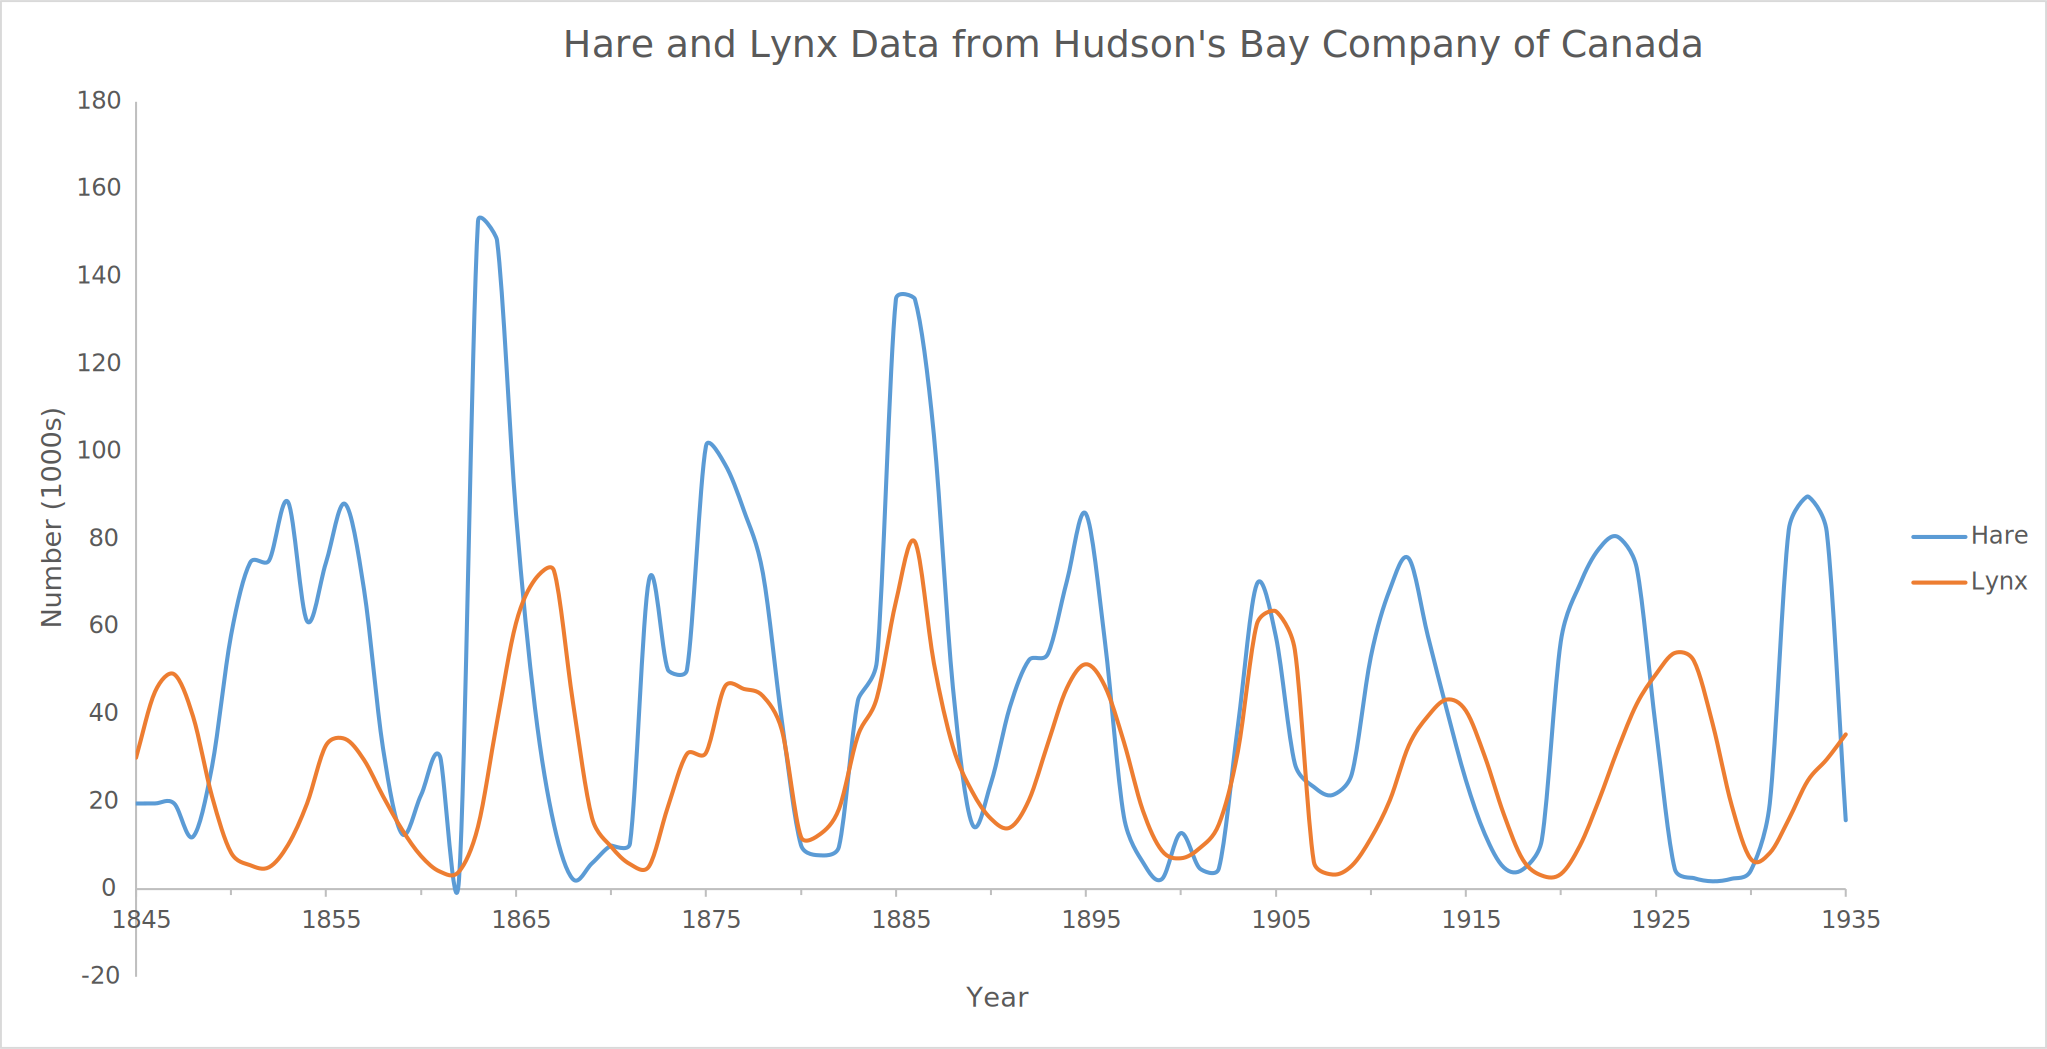
\includegraphics[width=\textwidth]{HareLynx.pdf}
	\caption{Hare and lynx data from Hudson's Bay Company (\href{https://www2.nau.edu/lrm22/lessons/predator_prey/predator_prey.html}{source}). Compare the periodic dynamics with the theoretic dynamics in \Cref{fig:lotkavolterra}.}
	\label{fig:harelynx}
\end{figure}

\subsection{Non-linear Methods}

We have seen how we can determine whether a critical point of a non-linear system is stable or unstable by using a linear approximation near the critical point. However, there are certain limitations to these methods, such as that the Jacobian may not give us any information about the system (e.g. when it is the zero matrix, as in \Cref{eg:lyapunov2}), or the critical point of the linearisation may be a centre, as was the case in the damped pendulum example (\Cref{eg:dampedpendulum2}) and the Lotka-Volterra Model of \Cref{sec:lotkavolterra}.

Therefore, we now develop methods that apply directly to analyse non-linear systems of ODEs.

\subsubsection{Lyapunov Methods}

For motivation, consider a particle on a one-dimensional landscape with variable height $h(x)$. Then the potential $V(x) = gh(x)$, where $g$ is the gravitational constant. Then by Newton's second law, $x'' = -V'(x)$.

We wish to transform this into a system of first-order ODEs, which we do via the usual method of defining a new variable $y=x'$, then $y' = x'' = -V'(x)$. So we have the following system:
\begin{align*}
	x' &= y \\
	y' &= -V'(x).
\end{align*}

From here, it is easy to see that the critical points occur when $y=0$ and $V'(x)=0$. In other words, the CP is $(x_*, 0)$ with $V'(x_*) = 0$. To see what information we can find about this critical point via the linearisation, we calculate the Jacobian:
\[
J = \mat{0 & 1 \\ -V''(x) & 0} \implies J\mid_{(x_*,0)} = \mat{0 & 1 \\ -V''(x_*) & 0}
\]
The characteristic equation of the Jacobian at the CP is
\[
r^2 + V''(x_*) = 0.
\]

Therefore, if $x_*$ is a minimum of $V(x)$ (so $V''(x)>0$),
\[
r = \pm i\sqrt{V''(x_*)},
\]
and the critical point of the linear system is a centre.

If $x_*$ is a maximum of $V(x)$ (so $V''(x)<0$),
\[
r = \pm \sqrt{-V''(x_*)},
\]
and the critical point is a saddle point, which is unstable.

Therefore, in the case that $x_*$ is a minimum of $V$, we cannot conclude about the (in)stability of the non-linear system based on the centre of the linear system. So what can we say about the system that is not limited to the behaviour of the linearised system near the critical points?

What we can do is define the following function $F$ which is time-invariant (the physics interpretation is that $F$ is the sum of kinetic and potential energy):
\[
F(x,y) = \frac{y^2}{2} + V(x).
\]
Then
\[
\frac{dF}{dt} = yy' + V'(x)x' = -yV'(x) + V'(x)y = 0.
\]
Therefore $F$ is constant along trajectories, which corresponds to our idea of it representing energy which is of course conserved (in an isolated system). Thus, we can also say that the trajectories are constant level curves of $F$.

Now, we define the function
\[
E(x,y) = F(x,y) - F(x_*,0) = \frac{y^2}{2} + V(x) - V(x_*).
\]

\begin{remark}
	$E$ is called a Lyapunov Function.
\end{remark}

Observe that $E(x_*, 0)=0$, $\frac{dE}{dt} = 0$, and that if $x_*$ is a minimum of $V$, $E(x,y) \geq 0$. On the other hand, if $x_*$ is a maximum, then $E$ is sign-indefinite, corresponding to a saddle point at the CP $(x_*,0)$.

Therefore in the case of the minimum, the level curves for $E$ are closed and bounded, giving a stable equilibrium that looks something like a centre.

To summarise, we found an implicit function $E$ with $\frac{dE}{dt} = 0$\footnote{Also works if $\frac{dE}{dt}<0$ or $\frac{dE}{dt}\leq0$} and $E \geq 0$, where the existence of this function implies that the critical point $(x_*,0)$ is stable. This idea is the foundation of Lyapunov's method.

Thus, we are now ready to state the formal definitions and methods relating to the Lyapunov Methods.

\begin{definition}
	$E(x,y)$ is positive definite if $E(x,y)>0$ for all $(x,y) \neq (0,0)$. Similarly, $E(x,y)$ is positive semi-definite if $E(x,y)\geq 0$ for all $(x,y) \neq (0,0)$.
\end{definition}

\begin{theorem}[Lyapunov Stability Theorem]\label{thrm:lyapunov1}
	If there exists a positive definite $E(x,y)$ such that $\frac{dE}{dt}$ is negative definite (semi-definite) on some domain $D$ containing the origin, then $\xta = (0,0)$ is asymptotically stable (stable).
\end{theorem}

\begin{theorem}[Lyapunov Instability Theorem]\label{thrm:lyapunov2}
	Suppose there exists $E(x,y)$ such that $E(0,0)=0$, and in every neighbourhood of the origin there is at least one point where $E$ is positive (negative). If there exists a domain $D$ containing the origin such that $\frac{dE}{dt}$ is positive definite (negative definite) on $D$, then the origin is an unstable critical point.
\end{theorem}

With the Lyapunov methods, we can see that, once we have a valid Lyapunov function $E$, it is not difficult to show that the conditions of Theorems \ref{thrm:lyapunov1} or \ref{thrm:lyapunov2} hold and therefore make conclusions on the stability/instability of the critical point. The difficult part of this process is finding the Lyapunov function $E$ in the first place.

To illustrate the application of these theorems, we consider the following examples.

\begin{eg}
	We have the system\footnote{Note that since this is a linear system, we can determine the stability of the critical points using the usual Jacobian-eigenvalue method. But that would ruin the fun of using our new-found theorems.}
	\begin{align*}
		x' &= -2x \\
		y' &= x-y.
	\end{align*}
	
	Fortunately, we have a flash of inspiration and decide to try
	\[
	E(x,y) = ax^2 + by^2, \quad a,b>0,
	\]
	where $E(x,y)>0$ for $(x,y)\neq(0,0)$.
	
	Using the chain rule,
	\begin{align*}
		\frac{d}{dt}E = 2axx' + 2byy' &= -4ax^2 + 2by(x-y) \\
		&= -2b\left(\frac{2a}{b}x^2 - xy + y^2\right) \\
		&= -2b\left(\frac{x}{2} - y\right)^2 \leq 0,
	\end{align*}
	where we pick $a$ and $b$ such that $\frac{2a}{b} = \frac14$ in order to factorise the second line.
	
	Therefore $E$ is positive definite and $E'$ is negative semi-definite, so by \Cref{thrm:lyapunov1}, the CP $(0,0)$ is stable.
\end{eg}

\begin{eg}\label{eg:lyapunov2}
	We have the system
	\begin{align*}
		x' &= -xy^2 \\
		y' &= 3x^2y
	\end{align*}
	It is easy to see that $(0,0)$ is a critical point of this system. However, the Jacobian at $(0,0)$ is the zero matrix, which tells us nothing about the linearised system. So non-linear methods are required.
	
	We try the function
	\[
	E(x,y) = 3x^2 + y^2 > 0 \text{ for } (x,y) \neq (0,0).
	\]
	So $E$ is positive definite. Furthermore,
	\[
	\frac{dE}{dt} = 6xx' + 2yy' = -6x^2y^2 + 6x^2y^2 = 0,
	\]
	so $\frac{dE}{dt}$ is negative semi-definite and by \Cref{thrm:lyapunov1}, $\xta = (0,0)$ is stable.
\end{eg}

\begin{eg}
	We have the system
	\begin{align*}
		x' &= x+3y \\
		y' &= 2x.
	\end{align*}
	Try $E(x,y) = xy + by^2 > 0$ for some $(x,y)$. Also, $E(0,0)=0$.	Then
	\begin{align*}
		\frac{dE}{dt} = x'y + xy' + 2byy' &= (x+3y)y + 2x^2 + 4bxy \\
		&= 3y^2 + 2x^2 + xy(1+4b).
	\end{align*}
	Set $b=-\frac14$ so that $1+4b=0$, then $\frac{dE}{dt}$ is positive definite, and by \Cref{thrm:lyapunov2}, the critical point $(0,0)$ is unstable.
\end{eg}

\subsubsection{Poincar\'{e}-Bendixson Theorem}

We'll now move on to discuss the existence of periodic trajectories. 

The Poincaré-Bendixson theorem tells us when such periodic orbits exist. But what are periodic trajectories? To put it quite simply: any closed trajectory is a periodic trajectory.

If a solution is closed, then it repeats itself with a period $T$ which implies that there exists $T>0$ such that $\vbx(t+T) = \xt$. 
We've already encountered periodic trajectories around critical points which are centres. In this case, we had a family of periodic trajectories in the form of a collection of elliptical trajectories, each closed and periodic. However, we can also encounter cases of isolated periodic trajectories.

\begin{eg}\label{eg:periodicsol}
	\begin{align*}
		x' &= y - x(x^2 + y^2 - a^2) \\
		y' &= -x -y(x^2 + y^2 - a^2).
	\end{align*}
	First, we find the critical point to be at the origin $(0,0)$ and the Jacobian at this critical point is given by: 
	\[
	J(0,0) = \mat{a^2 & 1 \\ -1 & a^2}.
	\]
	The eigenvalues associated with $J(0,0)$ are found as follows: 
	\[
	(a^2 - r)^2 + 1 = 0 \implies r = a^2 \pm i.
	\]
	Since the eigenvalues are a pair of complex conjugates which are not purely imaginary, we have that $(0,0)$ is an unstable focus as $a^2 > 0$ and $r_1$ and $r_2$ are complex conjugates. So the critical point $(0,0)$ is a spiral source.
	
	But, does this trajectory spiral away to infinity or does it change its behaviour at some point? Let's have a look at the polar co-ordinates to understand this better:
	
	Let $x = r \cos{\theta}, y = r \sin{\theta}$. Then,
	\begin{align}
		\label{eq3.14}
		x' &= r' \cos{\theta} - r \theta' \sin{\theta} = r \sin{\theta} - r \cos{\theta}(r^2 - a^2) \\
		\label{eq3.15}
		y' &= r' \sin{\theta} + r \theta' \cos{\theta} = - r \cos{\theta} - r \sin{\theta}(r^2 - a^2).
	\end{align}
	Multiplying \Cref{eq3.14} by $\cos{\theta}$ and \Cref{eq3.15} by $\sin{\theta}$ and adding them together, we get:
	\[
	r' = -r(r^2 - a^2).
	\]
	Multiplying \Cref{eq3.14} by $-\sin{\theta}$ and \Cref{eq3.15} by $\cos{\theta}$ and adding them together, we get:
	\[
	r\theta' = -r.
	\]
	So, we now have a system of ODEs of the form:
	\begin{align*}
		r' &= -r(r^2 - a^2) \\
		\theta' &= -1.
	\end{align*}
	So, all the trajectories are going to rotate at a constant angular velocity 
	\[
	\theta = \theta_0 - t.
	\]
	We can also look at the dynamics in the radial direction separately as $r$ does not depend on $\theta$.
	
	\underline{Radial dynamics}: Since $r' = -r(r^2 - a^2)$, at $r=a$, we have a periodic trajectory as $r' = 0$ and when $r<a$, $r'$ is positive so $r$ is going to increase towards $a$ and when $r>a$, $r'$ is negative so $r$ is going to decrease towards $a$. The trajectories are illustrated in \Cref{fig:periodicsol} in the $a=1$ case.
\end{eg}

\begin{figure}[!ht]
	\centering
	\includegraphics[width=0.5\textwidth]{PeriodicSol.pdf}
	\caption{Trajectories of the system in \Cref{eg:periodicsol} when $a=1$. Observe that all trajectories spiral toward the red circle with $r=1$ as $t \to \infty$ \cite[Figure 9.7.1]{boyce}.}
	\label{fig:periodicsol}
\end{figure}

The circle in the above example is an example of what is called a limit cycle.

\begin{definition}
	A limit cycle is a periodic solution such that at least one other non-closed trajectory tends to them as $t \to \infty$ or $t \to -\infty$ (or both).
\end{definition}

The limit cycle is (see \Cref{fig:limitcycles}): 
\begin{itemize}
	\item Asymptotically stable (or simply stable) if all nearby trajectories tend to it as $t \to \infty$.
	\item Asymptotically unstable (or simply unstable) if all trajectories go away from the limit cycle as $t \to \infty$.
	\item Semi-stable (or half-stable) when trajectories tend to the limit cycle from one side but move away from the limit cycle from the other side.
\end{itemize}

The example in \Cref{eg:periodicsol} was asymptotically unstable.

\begin{figure}[!ht]
	\centering
	\includegraphics[width=0.9\textwidth]{LimitCycles.png}
	\caption{Graphical representation for each of the three types of limit cycle \cite{limitcycles}.}
	\label{fig:limitcycles}
\end{figure}

\subsubsection*{Existence of limit cycles and periodic trajectories}

Consider a set of autonomous functions $F$ and $G$ which are continuously differentiable on a domain $D$.

\begin{theorem}\label{thrm:periodictraj1}
	A closed trajectory must enclose at least one critical point. If this critical point is unique, then it cannot be a saddle point.
\end{theorem}

\begin{proof}
	While the mathematical proof will not be discussed here, the topological reasoning might be helpful. 
	The uniqueness of the critical point implying that the critical point cannot be a saddle point holds because if we do imagine a saddle point surrounded by a periodic trajectory, it could look something like \Cref{fig:cpnosaddle} where $A$ is the saddle point but $B$ and $C$ could be other critical points which then contradicts that $A$ is the only critical point.
\end{proof}

\begin{figure}[!ht]
	\centering
	\includegraphics[width=0.55\textwidth]{CPNoSaddle.pdf}
	\caption{In this example, the trajectories are \href{https://mathworld.wolfram.com/CassiniOvals.html}{Cassini ovals}.}
	\label{fig:cpnosaddle}
\end{figure}

The negative version of this theorem is more useful:

\begin{theorem}\label{thrm:periodictraj2}
	Assume $\p_x F(x,y) + \p_y G(x,y) \neq 0$ in a simply connected domain $D$, then there are no periodic trajectories in $D$.
\end{theorem}

\begin{proof}
	A simply connected two-dimensional domain is one with no holes. If you've not already noticed, $\p_x F(x,y) + \p_y G(x,y)$ is the divergence of (F,G). Divergence is the measure of contraction or expansion of an area under the vector field, as in \Cref{fig:divergence}.
	
	\begin{figure}[!ht]
		\centering
		\includegraphics[width=0.8\textwidth]{Divergence.pdf}
		\caption{(Left to right) Positive, negative, and zero divergence of a vector field at a point (source: \href{https://commons.wikimedia.org/wiki/File:Divergence_(captions).svg}{Wikimedia}).}
		\label{fig:divergence}
	\end{figure}
	
	In fact, by Green's theorem,
	\[
	\frac{dA}{dt} = (\p_x F + \p_y G)A.
	\]
	In other words, the rate of change of an area is given by the divergence of the vector field times the area.
	
	Now, if you have a closed trajectory, the area inside is going to evolve into itself. So, the rate of change of the interior of this trajectory should be zero. Thus, if the area is increasing (or decreasing) because $(\p_x F + \p_y G) \neq 0$, then the closed trajectory would expand (or contract) and so, it cannot be invariant under the ODEs.
\end{proof}

\begin{remark}
	Note that the above two theorems help to rule out trajectories that are not periodic rather than prove that they are periodic.
\end{remark}

\begin{eg}
	We work with the same system as in \Cref{eg:periodicsol}:
	\begin{align*}
		x' &= y - x(x^2 + y^2 - a^2) = F(x,y) \\
		y' &= -x - y(x^2 + y^2 - a^2) = G(x,y).
	\end{align*}
	Then, 
	\begin{align*}
		\p_x F + \p_y G &= -(x^2 + y^2 - a^2) - 2x^2 - (x^2 + y^2 - a^2) - 2y^2 \\
		&= -4x^2 - 4y^2 + 2a^2 \\
		&= -4r^2 + 2a^2.
	\end{align*}
	
	So for $r < \frac{a}{\sqrt{2}}$, $\p_x F + \p_y G > 0$. Therefore, there is no periodic trajectory in this region by \Cref{thrm:periodictraj2}.
	
	We already know from the earlier example that $r$ has no periodic trajectory when $0<r<a$, so this theorem is not the most optimum one we can use, but it still offers some idea of a region in the phase plane that does not have a periodic trajectory. 
\end{eg}

\begin{theorem}[Poincar\'{e}-Bendixson theorem]
	Consider $D_1 \subset D$. Let the functions $F$ and $G$ have continuous first partial derivatives in a domain $D$ of the $xy$-plane and $R := D_1 \cup \p D_1$ (where $\p D_1$ is the boundary of $D_1$). Suppose there are no critical points in $R$ and there exists a trajectory $(x(t),y(t)) \in R$ for all $t$. Then either $(x(t),y(t))$ is periodic or it tends to a periodic trajectory.
\end{theorem}

\begin{remark}
	From \Cref{thrm:periodictraj1}, when we have a region enclosed by a periodic trajectory, then there exists a critical point somewhere in the region. So, to make the Poincaré-Bendixson theorem valid, we have to show that there is no critical point, yet there exists a periodic trajectory. So, $R$ should not be simply connected and must contain a hole at the critical point so that both \Cref{thrm:periodictraj1} and the Poincaré-Bendixson theorem hold.
\end{remark}

\begin{remark}
	The key to using the theorem is not to find a trajectory that does not leave the domain, but rather to find a trapping region $R$ such that once a trajectory enters the region, it never leaves.
	
	So, to prove that $R$ is a trapping region, we show that the vector field is pointing toward the interior of the domain $R$ everywhere, e.g. as in \Cref{fig:trappingregion}.
\end{remark}

\begin{figure}[!ht]
	\centering
	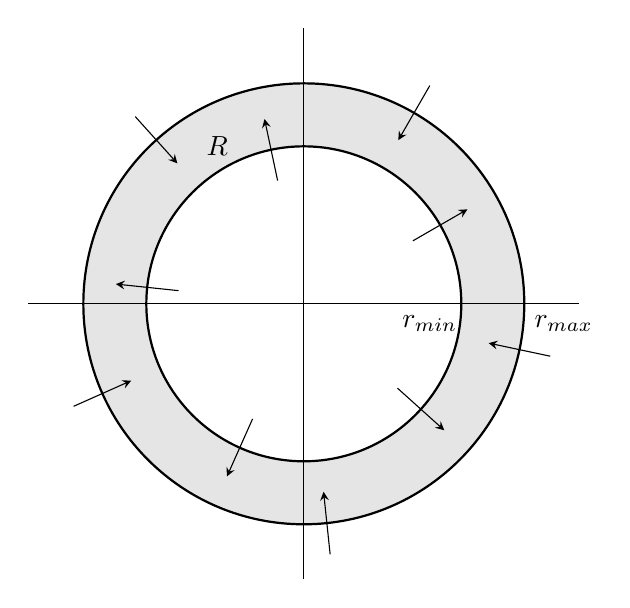
\begin{tikzpicture}
		\filldraw[color=black, fill=gray!20, thick] (0,0) circle (2.8);
		\filldraw[color=black, fill=white, thick] (0,0) circle (2);
		\draw (-3.5,0) -- (3.5,0);
		\draw (0,-3.5) -- (0,3.5);
		\node at (1.6,-0.25) {$r_{\text{min}}$};
		\node at (3.3,-0.25) {$r_{\text{max}}$};
		\node at (-1.1, 2) {$R$};
		\foreach \x in {0,...,4}{
			\draw[-stealth] (30+72*\x:1.6) -- (30+72*\x:2.4);
			\draw[-stealth] (60+72*\x:3.2) -- (60+72*\x:2.4);
		}
	\end{tikzpicture}
	\caption{An example of a trapping region $R$, where the vector field always points towards the interior of $R$.}
	\label{fig:trappingregion}
\end{figure}

\begin{eg}
	Returning to the system from \Cref{eg:periodicsol} where we found
	\[
	r' = -r(r^2 - a^2),
	\]
	let $R = {\frac{a}{2}<r<2a}$. Then, $r' > 0$ for $r = \frac{a}{2}$ and $r'<0$ for $r = 2a$.
	
	Thus, $R$ is a trapping region (essentially looking like \Cref{fig:trappingregion}). There are no critical points in this region as $(0,0)$ is the only critical point for the system which is not included in the trapping region $R$. So by the Poincaré-Bendixson theorem, there exists a periodic trajectory in $R$.
\end{eg}

\begin{eg}
	Consider the system
	\begin{align*}
		x' &= y \\
		y' &= -x + y(1-3x^2-2y^2).
	\end{align*}
	To find whether a limit cycle exists in this system, let $r^2 = x^2 + y^2$. Then,
	\begin{align*}
		rr' & = xx' + yy' \\
		& = xy - xy + y^2(1-3x^2-2y^2) \\
		& = y^2(1-3x^2-2y^2).
	\end{align*}
	So, 
	\[
	rr' \geq y^2(1 - 3x^2 - 3y^2) \geq y^2(1-3r^2) \geq 0 
	\] if $r \leq \frac{1}{\sqrt{3}}$
	and
	\[
	rr' \leq y^2(1 - 2x^2 - 2y^2) \leq y^2(1-2r^2) \leq 0 
	\] if $r \geq \frac{1}{\sqrt{2}}$.
	
	Thus, a trapping region is given by $R := \{r: \frac{1}{\sqrt{3}} \leq r \leq \frac{1}{\sqrt{2}}\}$\footnote{Since at the borders $r=\frac{1}{\sqrt{3}}$ and $r=\frac{1}{\sqrt{2}}$, the trajectories point towards the interior of $R$ (or, at the very least, do not point outwards).} which does not include a critical point and by the Poincaré-Bendixson theorem, there exists a periodic trajectory in the system of ODEs.
\end{eg}